\documentclass{standalone}
\usepackage{tikz}
\usepackage{ctex,siunitx}
\setCJKmainfont{Noto Serif CJK SC}
\usepackage{tkz-euclide}
\usepackage{amsmath}
\usetikzlibrary{patterns, calc,3d}
\usetikzlibrary {decorations.pathmorphing,decorations.pathreplacing,decorations.shapes}
\begin{document}
\small
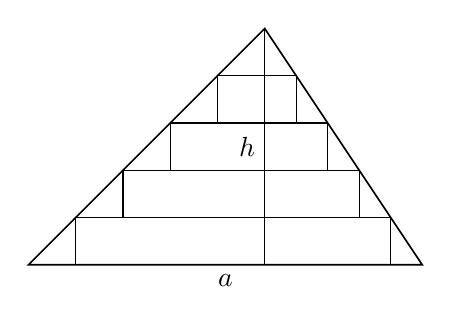
\begin{tikzpicture}[>=latex,scale=1.0]
  \draw[semithick](-3,0)--(2,0)node[midway,below]{$a$}--(0,3)--cycle;
  \draw(0,0)--(0,3)node[midway,left]{$h$};
  \foreach \x in {1,2,3,4}
  {
    \draw(-3+0.6*\x,0.6*\x)rectangle(2-0.4*\x,0.6*\x-0.6);
  }
\end{tikzpicture}
\end{document}